% !TeX root = project.tex
\newcommand*{\PathToAssets}{../assets}%
\newcommand*{\PathToOutput}{../_output}%
% \newcommand*{\PathToBibFile}{bibliography.bib}%

%%%%%%%%%%%%%%%%%%%%%%%%%%%%%%%%%%%%%%
%% This file is compiled with XeLaTex.
%%%%%%%%%%%%%%%%%%%%%%%%%%%%%%%%%%%%%%
\documentclass[12pt]{article}
%\documentclass[reqno]{amsart}
%\documentclass[titlepage]{amsart}
\usepackage{my_article_header}
\usepackage{my_common_header}
\usepackage{graphicx}

\begin{document}
\title{
Market Expectations in the Cross-Section of Present Values
}

\author{
Ilya Melnikov, Jared Szajkowski, Zac Johnson\
}
\begin{titlepage}
\maketitle

\doublespacing
\begin{abstract}
    Returns and cash flow growth for the aggregate U.S. stock market are highly and robustly predictable. 
    Using a single factor extracted from the cross-section of book-to-market ratios, 
    we find an out-of-sample return forecasting R\textsuperscript{2} of 13\% at the annual frequency (0.9\% monthly). 
    We document similar out-of-sample predictability for returns on value, size, momentum, and industry portfolios. 
    We present a model linking aggregate market expectations to disaggregated valuation ratios in a latent factor system. 
    Spreads in value portfolios’ exposures to economic shocks are key to identifying predictability and are consistent 
    with duration-based theories of the value premium.
\end{abstract}

\end{titlepage}


\doublespacing
\section{Out of Sample Regression Forecasts}

\begin{figure}[h]
    \centering
    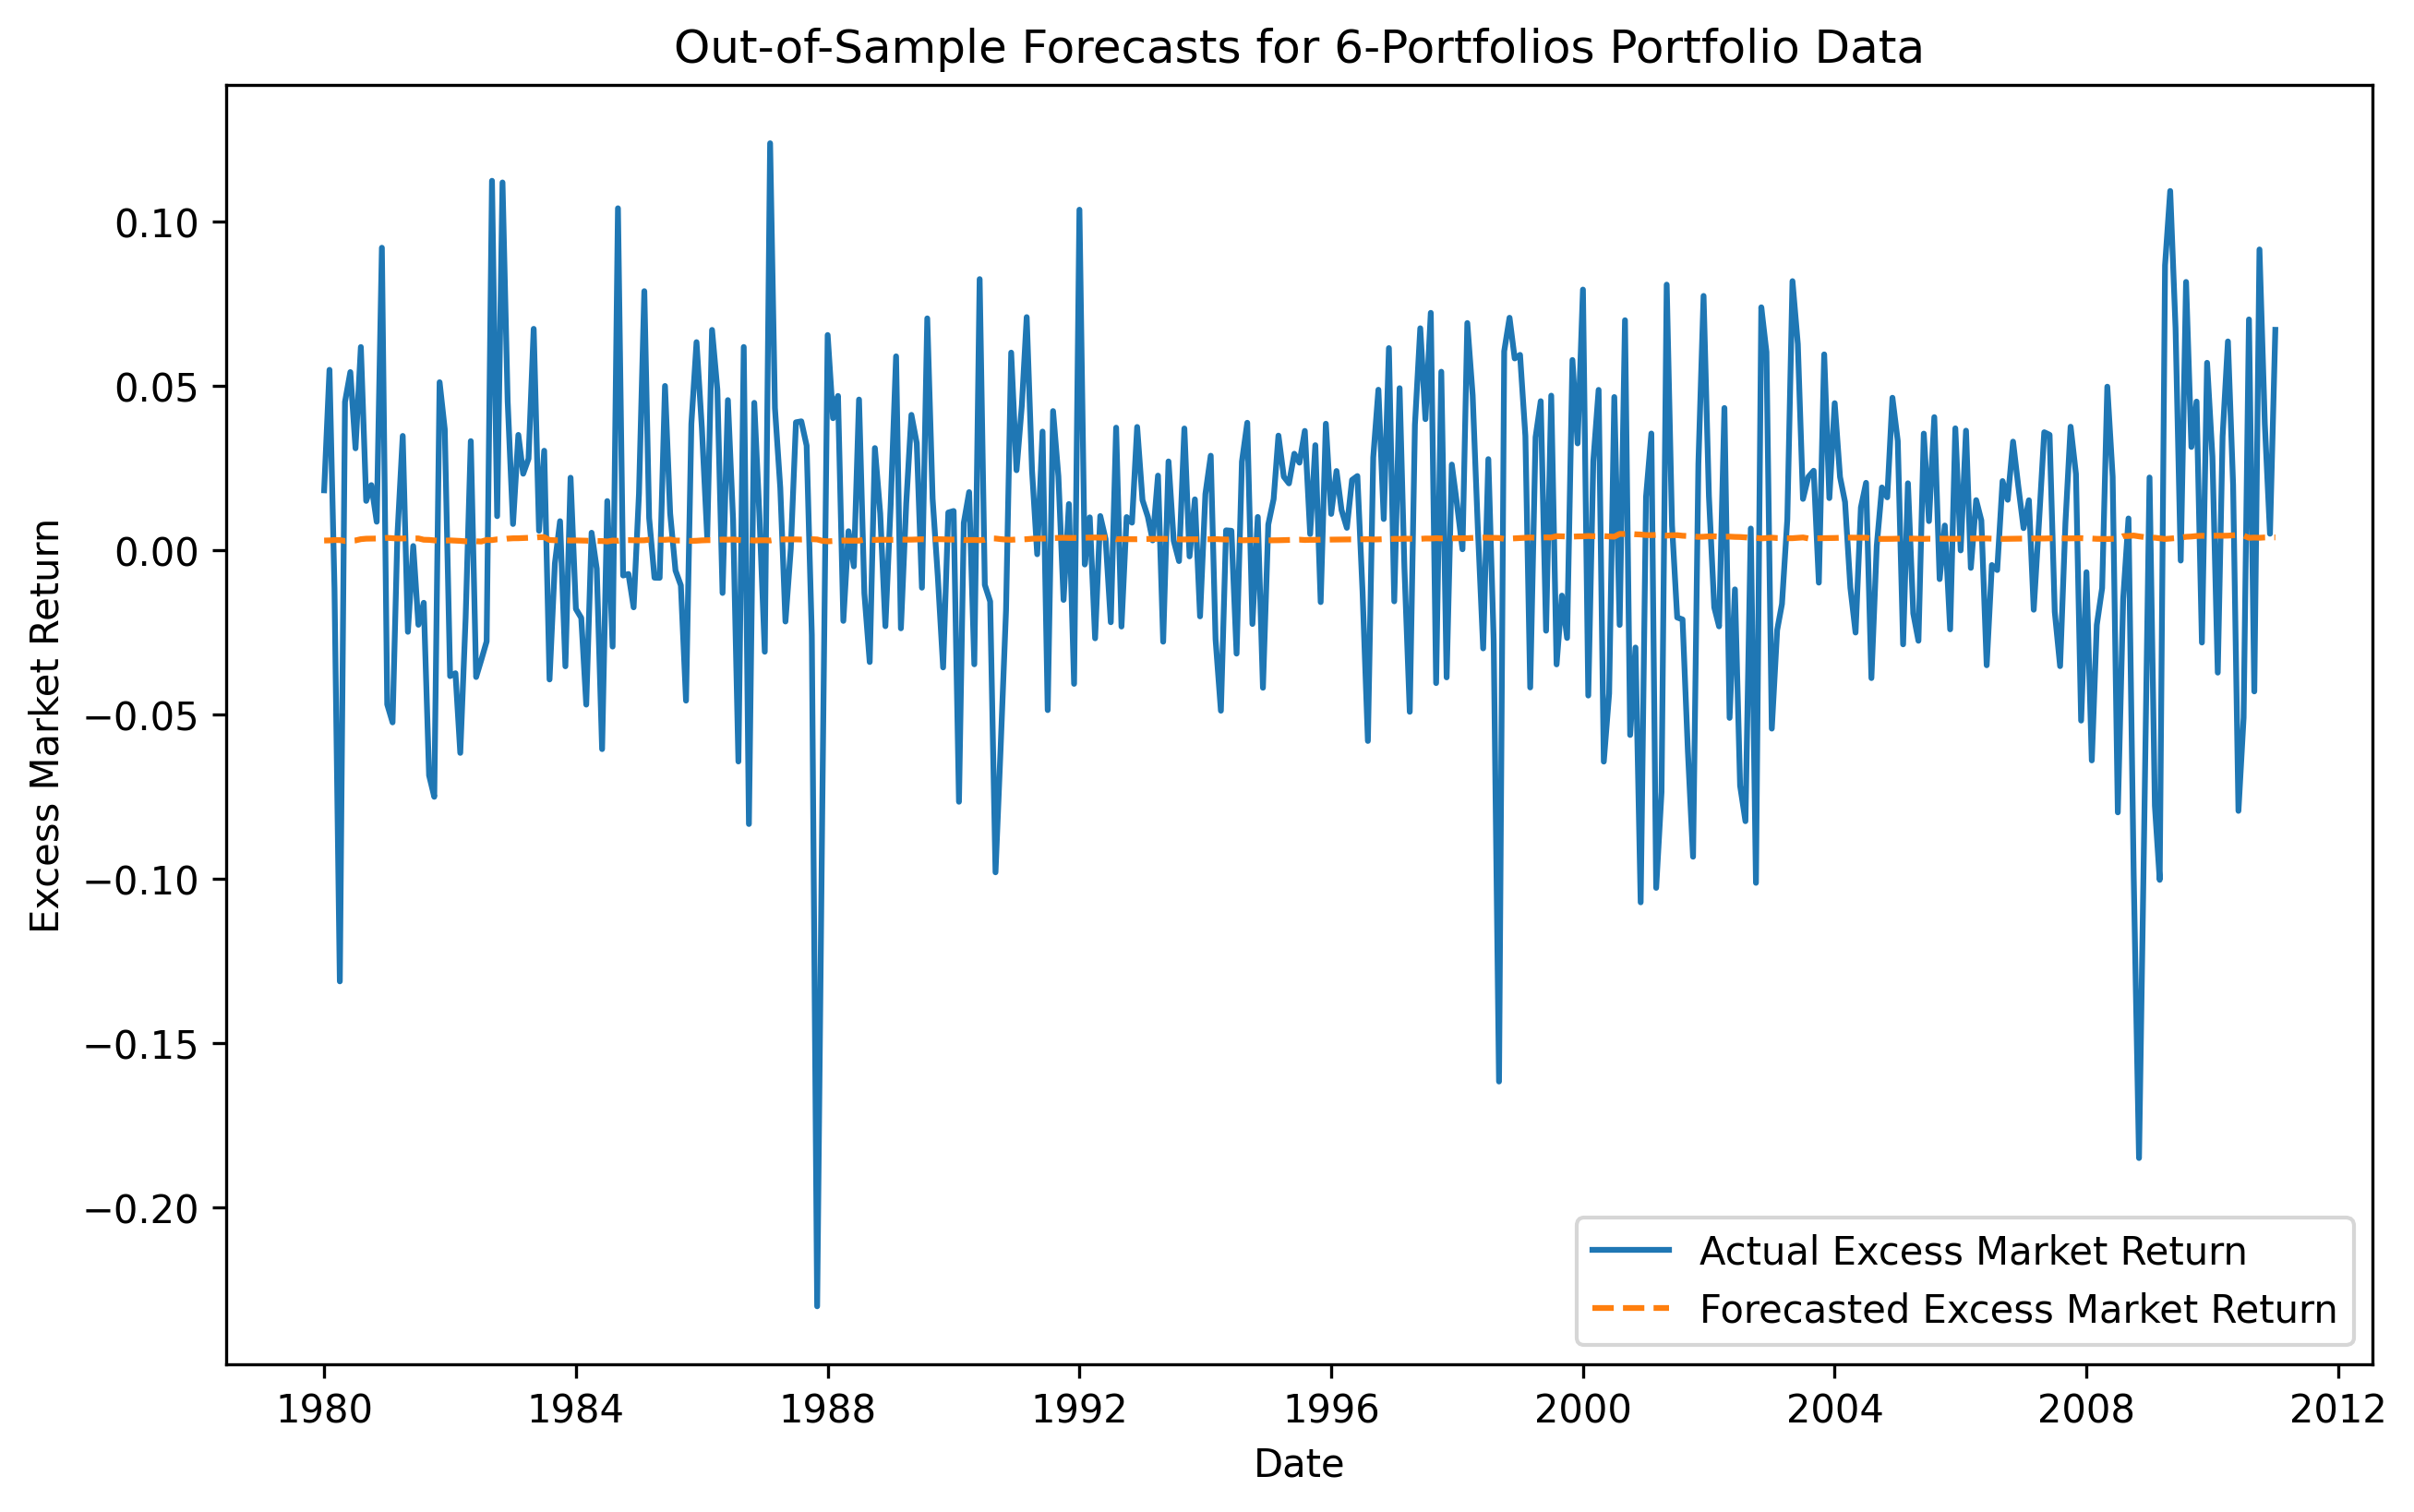
\includegraphics[width=0.8\textwidth]{plots/Out_of_Sample_Forecasts_for_6_Portfolios_Portfolio_Data.png}
    \caption{Out-of-Sample Forecast for 6-Portfolios Portfolio Data}
    \label{fig:forecast_chart}
\end{figure}

\begin{figure}[h]
    \centering
    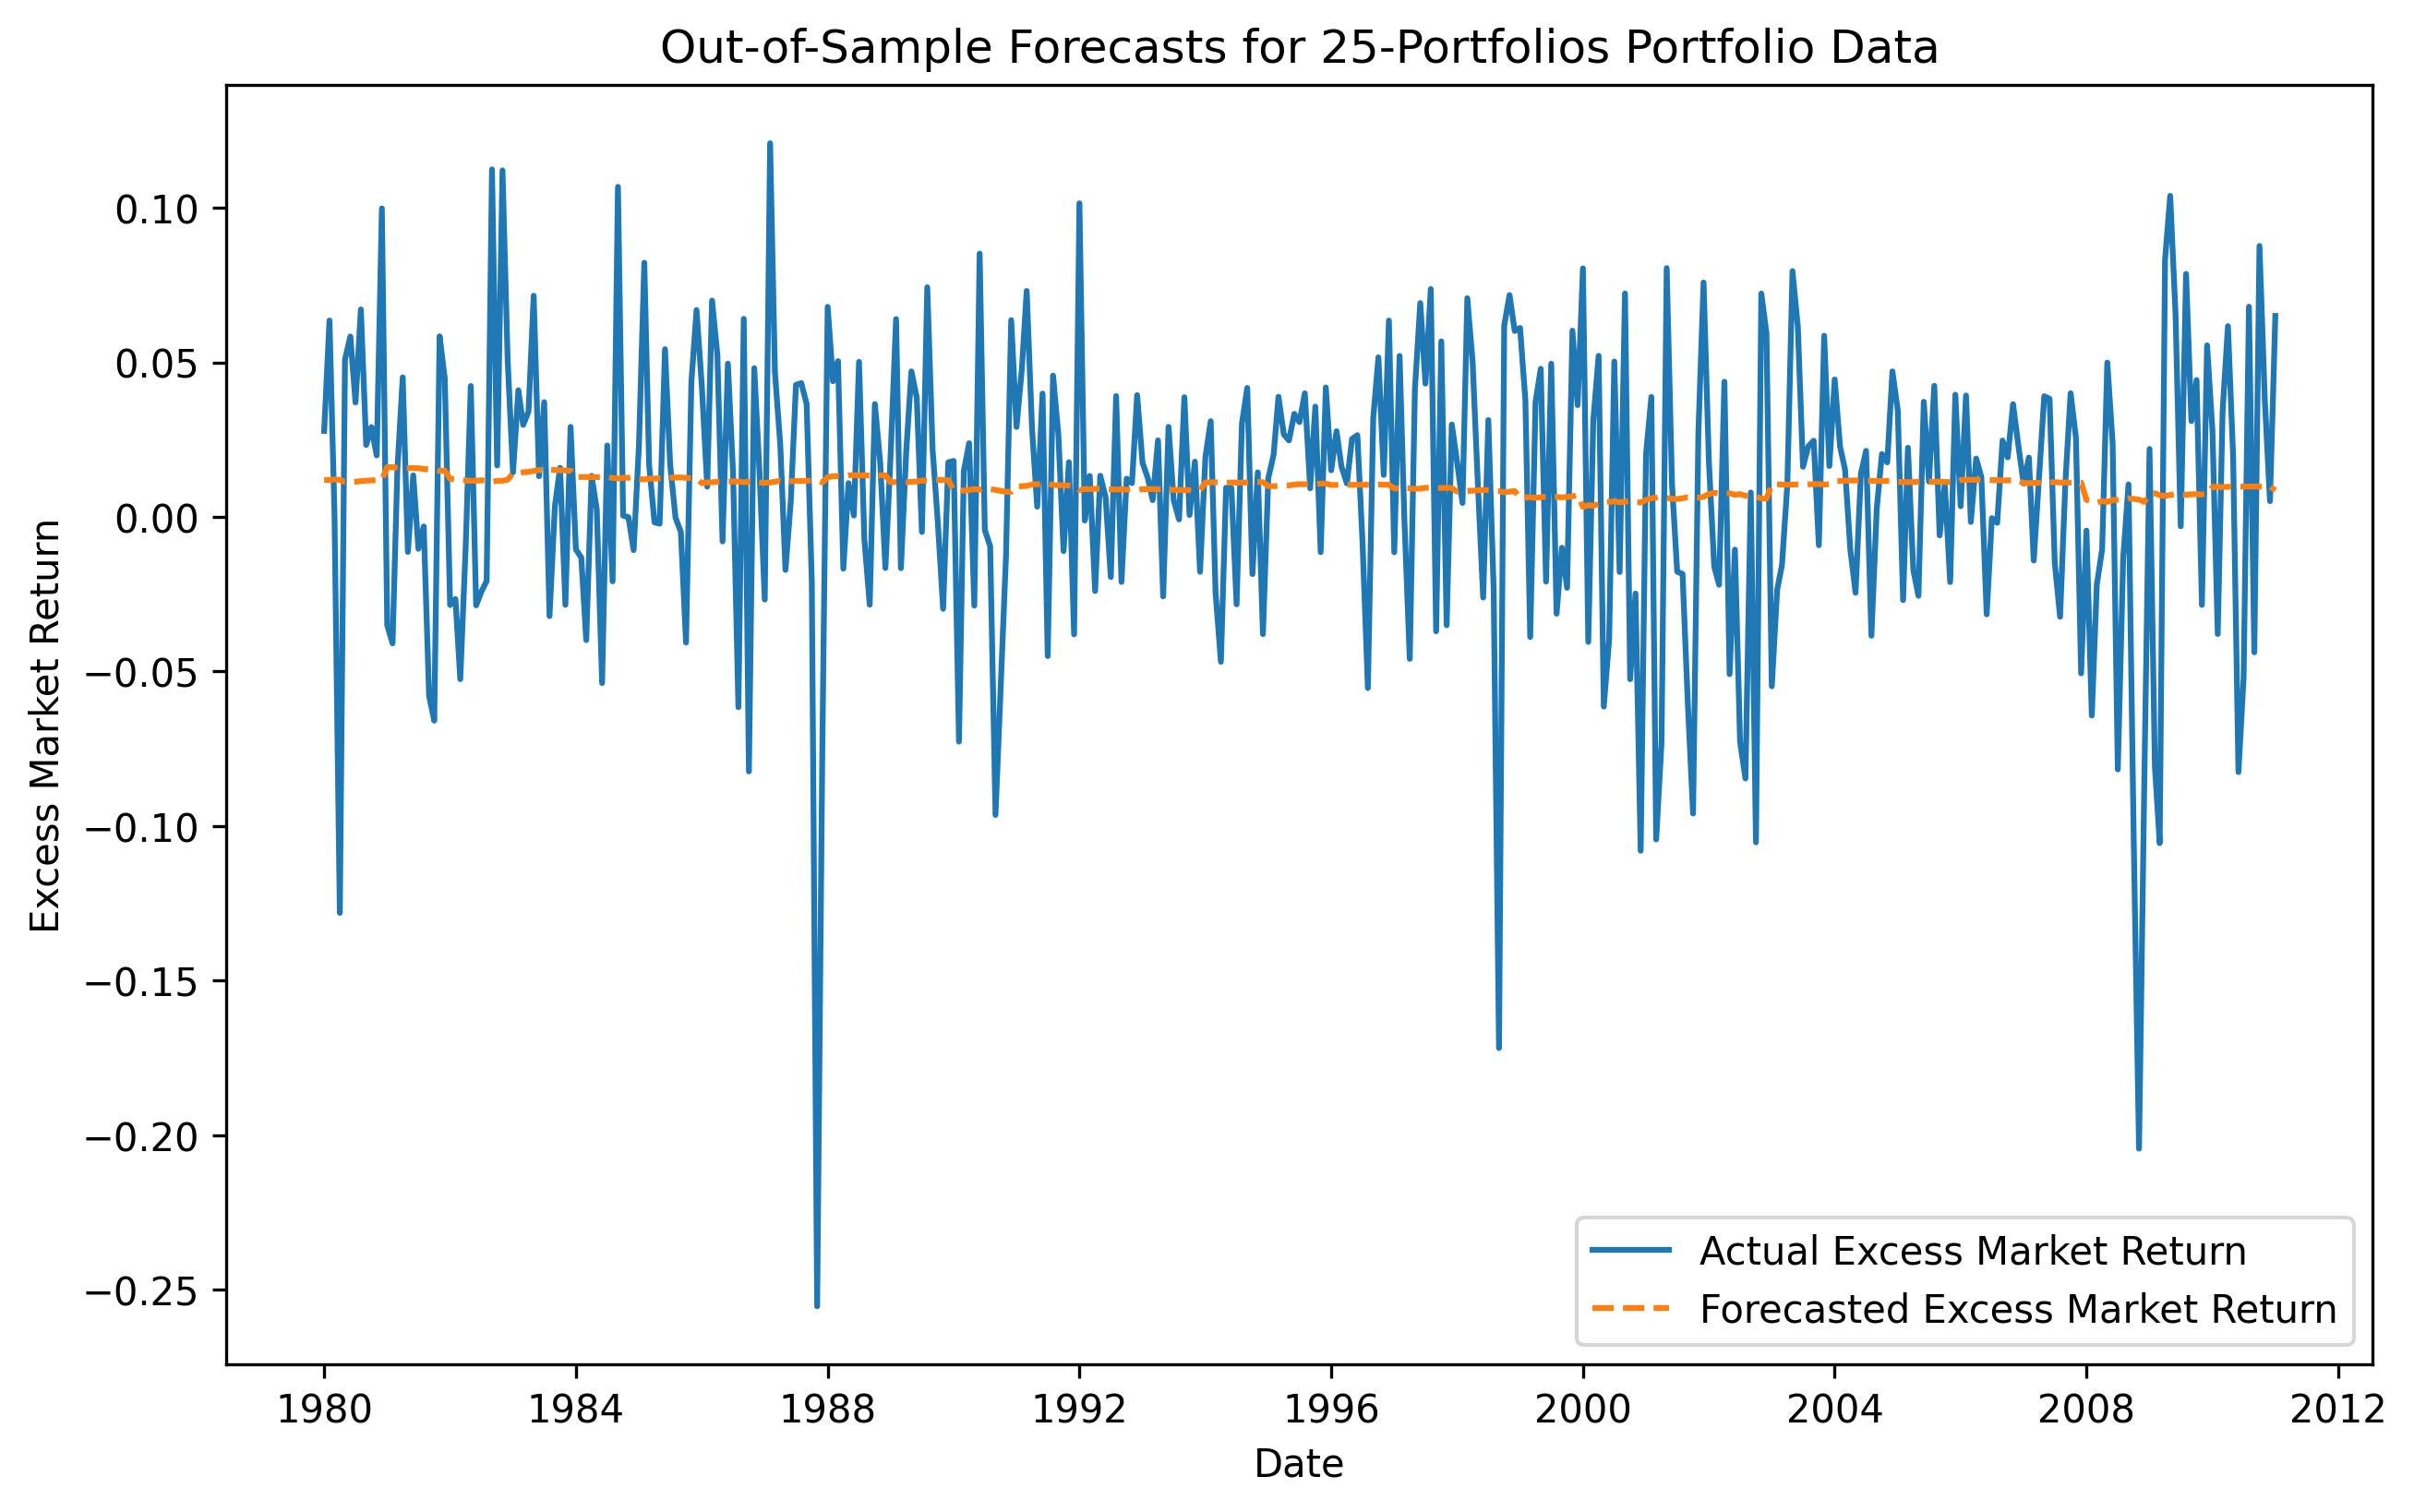
\includegraphics[width=0.8\textwidth]{plots/Out_of_Sample_Forecasts_for_25_Portfolios_Portfolio_Data.png}
    \caption{Out-of-Sample Forecast for 25-Portfolios Portfolio Data}
    \label{fig:forecast_chart}
\end{figure}

\begin{figure}[h]
    \centering
    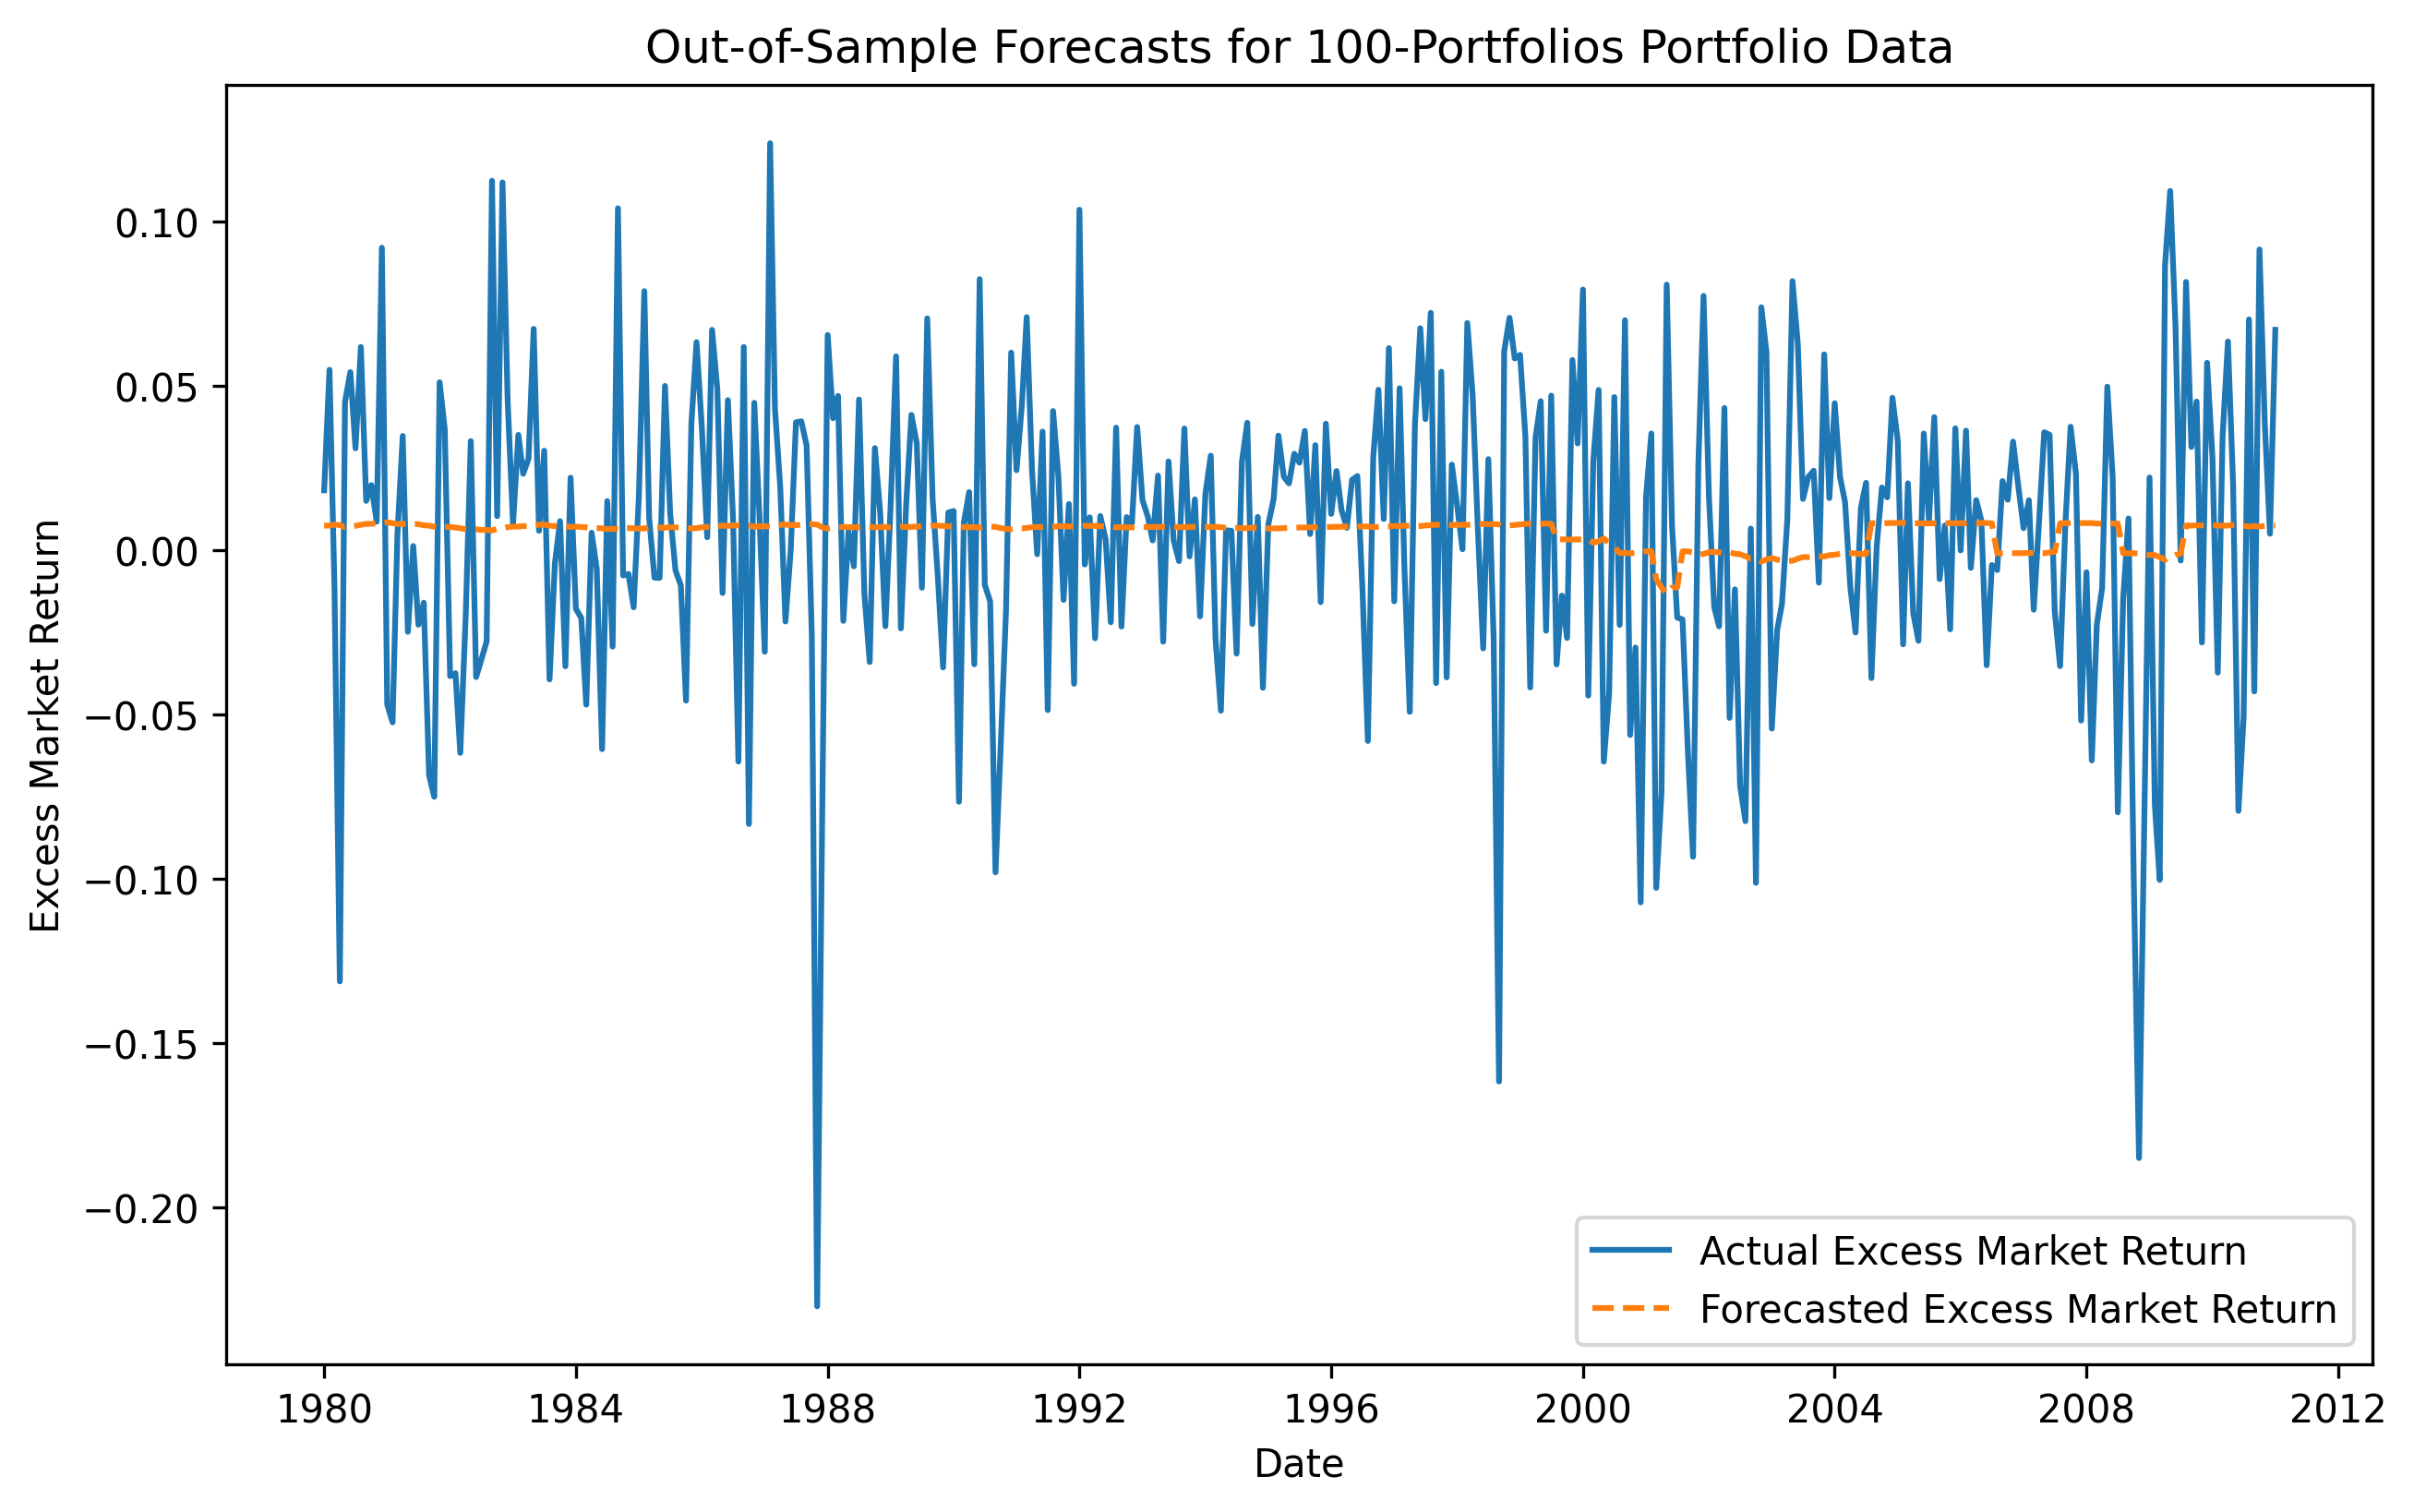
\includegraphics[width=0.8\textwidth]{plots/Out_of_Sample_Forecasts_for_100_Portfolios_Portfolio_Data.png}
    \caption{Out-of-Sample Forecast for 100-Portfolios Portfolio Data}
    \label{fig:forecast_chart}
\end{figure}


\doublespacing
\section{Out of Sample Regression Forecasts Results}
\begin{tabular}{lll}
\toprule
 & In-Sample R2 & Out-of-Sample R2 \\
\midrule
6 Portfolios In Sample & 0.017744 & NaN \\
25 Portfolios In Sample & 0.016459 & NaN \\
100 Portfolios In Sample & 0.019472 & NaN \\
6 Portfolios & NaN & -0.006179 \\
25 Portfolios & NaN & -0.005535 \\
100 Portfolios & NaN & -0.012337 \\
\bottomrule
\end{tabular}




\doublespacing
\section{Replication Overview}

The replication of Table 1 from Kelly and Pruitt (2013) aimed to validate the 
findings on market return predictability using book-to-market ratios. In this project we 
tried reconstructuring the key univariate predictor by applying partial least squares (PLS) 
to book-to-market ratios, with the goal of closely mirroring the original study’s results.

\doublespacing
\section{Successes}
Successfully accessed and processed CRSP and Compustat data to extract the relevant valuation 
ratios and market return data.
\\We have a great team. 



\doublespacing
\section{Challenges}

Data cleaning was time-intensive due to matching firm-level data from Compustat with 
returns from CRSP while ensuring proper alignment of fiscal periods.Academic Paper doesn't 
explicitely say how to shift the data for regressions. 
We've spent a lot of time trying to figure out how to line up the data with to match the R Squared
LaTex set up and getting used to took a bit of time. 


\doublespacing
\section{Data Sources}

CRSP: Provided market returns, stock prices, and trading volume data.
\\Compustat: Supplied firm-level fundamentals, including book-to-market ratios, 
which are essential for constructing valuation-based predictors.
\\Fama-French Factors: Used as a robustness check to compare return predictability against standard factor-based models.\par

\end{document}